\chapter{Monte Carlo simulations of designs}
\label{chapter:optimization}
\label{c6:monte-carlo}
In this chapter, Monte Carlo simulations of the instrument design variants performed using McStas \cite{willendrup2020} will be presented. The goal is to complement the analysis and constraints discussed in Chapter $\ref{c4:constraints}$ and provide an understanding of how instruments might behave in practice for a range of samples and how measurement data can be analysed. 

% after all the analysis and discussion of constraints/optimizing using these, introduce monte carlo simulations as a step closer to a practical instruments and a way to verify identified limitations and see them in play. This last aspect could be an interesting part of the discussion of simulation results as well, you can really point out narrowing modulation envelopes, modulation periods becoming too big for the detecto retcetera. 
% I expect some designs to not be able to measure specific samples at all or barely to the extent that showing them in a plot is a bit silly. 

\section{Method}
To test the ability of the various instruments to measure samples in the characteristic length range of $\SI{10}{\nano\meter}$ to $\SI{5}{\micro\meter}$ three samples of the type described in Section \ref{c2.4} are considered with radii $R = \SI{50}{\nano\meter}, \SI{300}{\nano\meter}, \SI{2}{\micro\meter}$. Although these could in principle all be simulated with other sample parameters like sample thickness $t$ the same, this would cause the scattering power $\tau$ as defined in Equation \eqref{eq:sample-tau} to vary greatly and cause it to go too far out of the range of $0.1$ and $0.8$ that is typically considered to be optimal in terms of signal-to-noise ratio \cite{bouwman2021b}\cite{heijkamp2011}. For this reason, $t$ is varied between $1 - 10 ~\unit{\milli\meter}$ for different $\lambda_0, R$ pairings to optimize $\tau$. The remaining sample parameters take values $\phi = 0.015$, $\Delta\rho = \SI{1.8e10}{\centi\meter}^{-2}$ and are the same in each case. The chosen $t$ values with the corresponding $\tau$ are shown in Table \ref{tab:sample-thickness}.

\begin{table}[h!]
	\centering
	\begin{tabular}{cc|cc}
		\toprule
		$\lambda_0~[\unit{\angstrom}]$  & $R ~[\unit{\nano\meter}]$  & $t ~[\unit{\milli\meter}]$& $\tau~[\unit{\meter^3}]$ \\
		\midrule
		\num{4.321} & \num{50} & \num{10} & \num{0.067}\\
		\num{4.321} & \num{300} & \num{10} & \num{0.4022} \\
		\num{4.321} & \num{2000} & \num{1} & \num{0.2681} \\
		\num{8} & \num{50} & \num{10} & \num{0.2298} \\
		\num{8} & \num{300} & \num{5} & \num{0.6893} \\
		\num{8} & \num{2000} & \num{1} & \num{0.9191} \\
		\bottomrule
	\end{tabular}
	\caption{Combinations of $\lambda_0$ and sample radius $R$ with a sample thickness $t$ chosen to keep $\tau$ approximately within the optimal range of $0.1$ and $0.8$.}
	\label{tab:sample-thickness}
\end{table}

\subsection{Simulated measurement procedure}
For each instrument as described in Table \ref{tab:design-variants}, measurements on the three samples with radii and thicknesses as given in Table \ref{tab:sample-thickness} were simulated. Additionally, an empty measurement was done for each instrument to establish a baseline. 

To perform a measurement, a range of $B$-field strength values is simulated with the analyser in the $+x$ and $-x$ settings. Although in principle the full range of $B$-values bounded by the focussing condition could be simulated, only $B$-values were considered that correspond to the respective instrument $\delta$-range as given in Table \ref{tab:designs-final-ranges} in Chapter \ref{c4:constraints}. The sample range was taken to be $\frac{R}{10} - 3R$ and the overlap between each instrument range and these sample ranges were computed. In each case there was overlap and 30 $B$-settings corresponding to the overlapping $\delta$-range were chosen. $B$-resolution limitations were not considered here but can in practice be expected to limit the number of practical measurements to fewer than 30 as well as introducing $\delta$ uncertainty, becoming especially relevant in the lower $\delta$ range. 

\subsection{Simulation setup}
To simulate the instruments, version 3.4 of the raytracing software package McStas \cite{willendrup2020} is used with OpenACC acceleration enabled. The simulations were performed on a desktop computer with an Intel Core i5-6600 quad-core 3.3 GHz CPU and an Nvidia GeForce GTX 1060 GPU. Simulated instruments are all derivative of the previously simulated \texttt{SEMSANS\_Delft} instrument \cite{bouwman2021b}. The \texttt{Foil\_flipper\_magnet} component was used to simulate foil flippers like in \texttt{SEMSANS\_Delft} and idealized components for the Wollaston prism and isosceles triangle were derived from the existing \texttt{Pol\_triafield} component. Each $B$-field and analyser setting was simulated using $10^7$ neutrons when using foil flippers and $10^8$ when using prisms or triangles. This due to the large difference in simulation time. Simulation time for a single simulation of $10^6$ varied from well under $\SI{1}{\second}$ for the prisms and triangles to about $\SI{4}{\second}$ for the foil flippers, presumably due to the greater complexity of the corresponding McStas component. 
The \texttt{SANS\_spheres2} sample component is used to model the described sample. Although most of its parameters correspond directly to those listed above, two that deserve mention are \texttt{Qmind} and \texttt{Qmaxd} which define the simulated $Q$-range. As the sample $R$ values span almost two orders of magnitude, the corresponding $Q$ range is quite different for the three samples and proportional to $1/R$. This is accounted for by using \texttt{Qmind}$=0.1/R$, \texttt{Qmaxd}$=10/R$, matching the sample $Q$-range as discussed in Section \ref{c2.4}.

\subsection{Data analysis}
To estimate $P(\delta) = e^{G(\delta)  - \tau}$, two data analysis methods are used on the simulation data. The first is based on fitting an expected modulation pattern as done elsewhere \cite{bouwman2011}\cite{parnell2023}, the second considers the RMS of the modulation pattern. The advantage of the second method is that it is more robust and better suited for real measurement conditions where many factors such as beam characteristics shape the observed modulation profile. Both rely on computing a quantity called the polarization $Pol(y)$\footnote{The choice for $Pol(y)$ instead of the more conventional $P(y)$ is deliberate and to avoid further overloading of $P$, which is already used in $P(\delta)$ and form factor $P(Q)$.}, defined as 
$$Pol(y) = \frac{I_{up}(y) - I_{down}(y)}{I_{up}(y) + I_{down}(y)}$$
Here $I_{up}, I_{down}$ correspond to simulated measurements using the $\pm x$ analyser settings. Intuitively, this gives a normalized expression for the modulation amplitude, allowing for some variation in total measured intensity $I_{up}(y) + I_{down}(y)$ across the detector. The signal at the boundaries of the detector is still not useful due to effects such as discussed in Section \ref{c4.4} and depicted in Figure \ref{fig:simplified-scattering} and only the middle $\SI{6}{\milli\meter}$ is used when estimating $P(\delta)$ for this reason.

In the first method, a modulation pattern with a Gaussian envelope similar to Equation \eqref{eq:poly-base-modulation} is fitted with variable amplitude to $Pol(y)$. Because $Pol(y)$ is used, $I_0$ disappears from the expression and $Pol_{b,s}(y)$ can largely be described by just $Pol_{\text{gauss}}(y) = A_{b,s}E(y)\cos(2\pi\alpha\lambda_0y)$ with fitted amplitudes $A_{b,s}$. In practice, a small error term $\epsilon$ is included to compensate for a potential non-zero average. This gives the final fitting function with parameters $A_{b,s}, \epsilon$
\begin{equation}
	Pol_{\text{fit}}(y) = \epsilon+ A_{b,s}E(y)\cos(2\pi\alpha\lambda_0y) \label{eq:gauss-fit-function}
\end{equation}
The resulting amplitudes $A_b, A_s$ with and without a sample at a given $B$ or $\delta$ setting are then related to $P(\delta)$ via $P_{exp}(\delta) = A_s/A_b$. 

In the second method, the RMS of $Pol(y)$ is computed as $RMS_{b,s}$ and again $P_{exp}(\delta)$ is given by the ratio $P_{exp}(\delta) = RMS_s/RMS_b$. The correctness of this method can be seen from the fact that for a single sinusoidal modulation the RMS is linearly proportional to the modulation amplitude. 

%As discussed in Section \ref{c3.6}, this can be expected to result in an error proportional to the width of the $\lambda$-spectrum, as a range of $\delta$'s is effectively sampled, each having their own $G(\delta)$ and $\tau(\delta)$. And as discussed in Sections \ref{c3.4} and \ref{c4.4}, the limited $Q$-range of the detector will result in incomplete detection of scattering for samples with smaller radii like $R = 50 \unit{\nano\meter}$ and a greater $Q$-range, limiting the accuracy of $G_\text{exp}(\delta)$. For these reasons, the value of $P(\delta)$ computed is to be understood as an estimate.  
\section{Results}
The result of the described simulation and data analysis using both methods is shown in Figures \ref{fig:simulation-plot-gauss}, \ref{fig:simulation-plot-rms}, with each subfigure showing simulated measurements within the accessible $\delta$-ranges for each design together with computed $P_{exp}(\delta)$ and analytical $P(\delta)$. Additionally, Figure \ref{fig:simulation-raw-intensity} shows an example of how raw simulation data from a simulated measurement using WP 8 is processed and fitted to $P_{exp}(\delta)$ in the two ways. The corresponding values are $P_{exp} = 0.52187 \pm 0.0002$ when using the Gauss method and $P_{exp} = 0.516 \pm 0.004$ when using the RMS. The analytical value is $P(\delta) = 0.501906$, which is incompatible with both estimates and their standard error. These values were computed from fitted amplitudes $A_b = 0.999905 \pm 8\cdot 10^{-6}$, $A_s = 0.5218 \pm 0.0002$ and RMS values $RMS_b = 0.9999226 \pm 4\cdot 10^{-7}$ and $RMS_s = 0.517 \pm 0.004$. In both cases, the uncertainty with a sample is much greater than without.
\begin{figure}[htbp]
	\centering
	\begin{subfigure}[b]{0.45\textwidth}
		\centering
		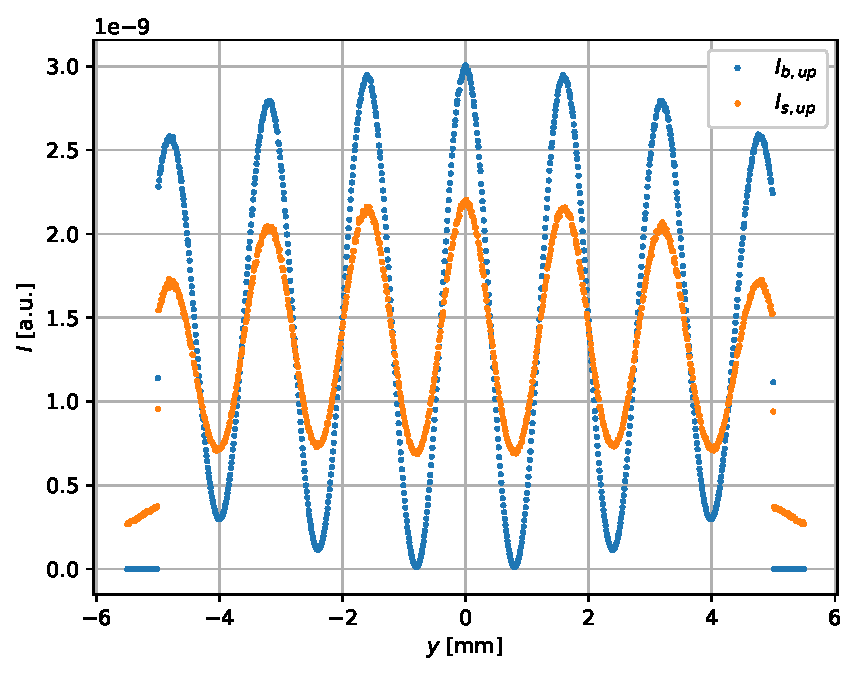
\includegraphics[width=\textwidth]{simulation-raw-intensity-up}
		\caption{$I_{b,up}$ and $I_{s,up}$ signals from }
		\label{fig:simulation-raw-intensity-up}
	\end{subfigure}
	\hfill
	\begin{subfigure}[b]{0.45\textwidth}
		\centering
		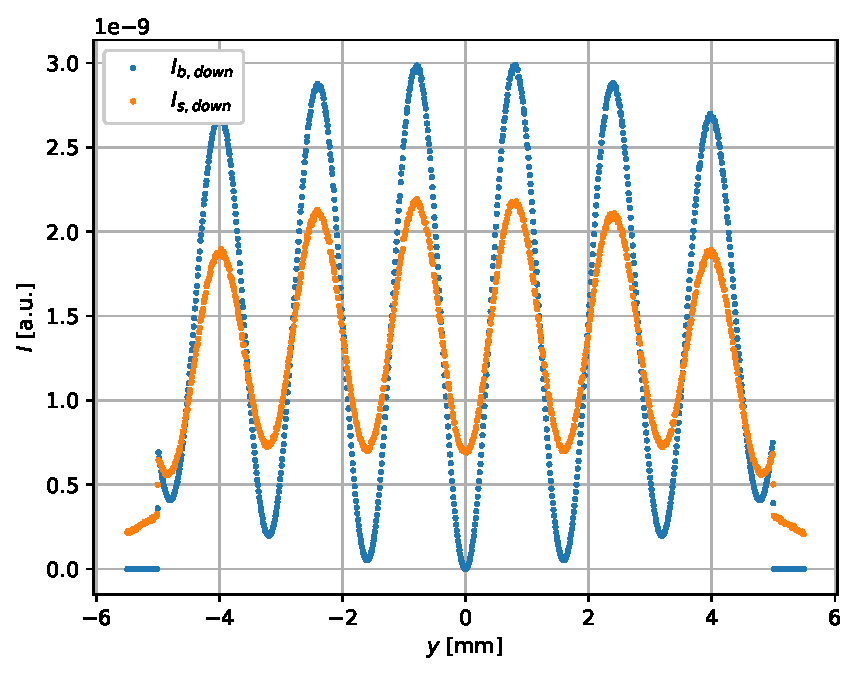
\includegraphics[width=\textwidth]{simulation-raw-intensity-down}
		\caption{$I_{b,down}$ and $I_{s,down}$}
		\label{fig:simulation-raw-intensity-down}
	\end{subfigure}
	\centering
	\begin{subfigure}[b]{0.45\textwidth}
		\centering
		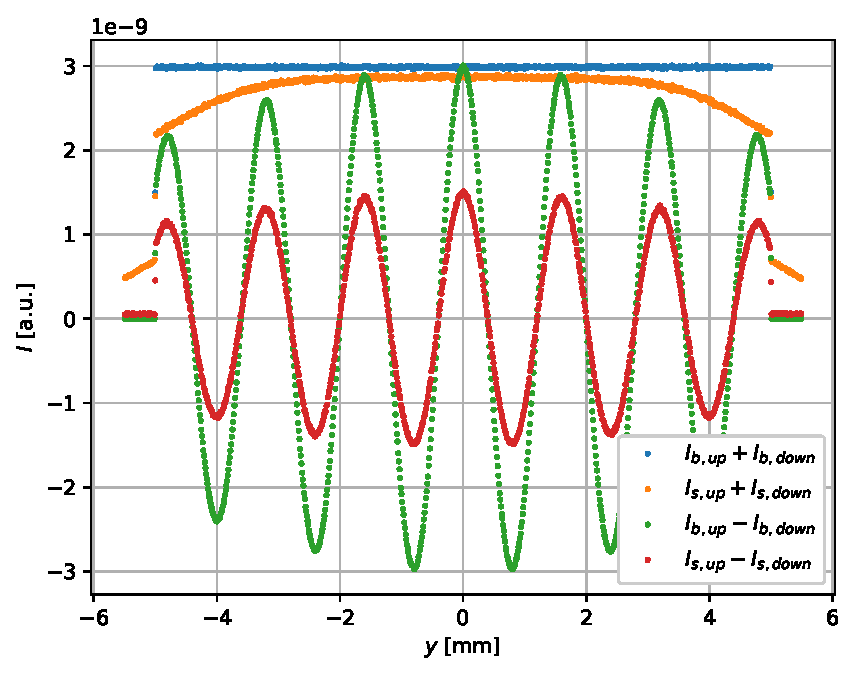
\includegraphics[width=\textwidth]{simulation-raw-intensity-differential}
		\caption{$I_{b,up} \pm I_{b,down}$ and $I_{s,up} \pm I_{s,down}$}
		\label{fig:simulation-raw-intensity-differential}
	\end{subfigure}
	\hfill
	\begin{subfigure}[b]{0.45\textwidth}
		\centering
		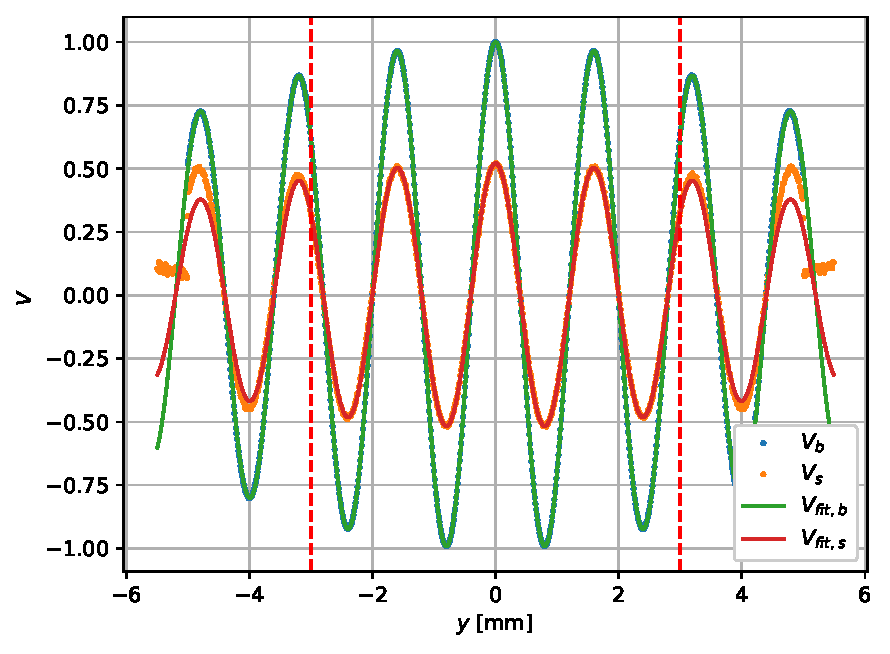
\includegraphics[width=\textwidth]{simulation-raw-intensity-pol}
		\caption{$Pol_b, Pol_s$ and fitted Gaussian modulations $Pol_{fit,b}, Pol_{fit,s}$}
		\label{fig:simulation-raw-intensity-pol}
	\end{subfigure}
	\caption{An illustration of the detector intensity patterns recorded during simulations and how they are processed to a fit. The data corresponds to a simulated measurement using WP 8 of the $R = \SI{300}{\nano\meter}$ sample with $B_1 = \SI{5.4}{\milli\tesla}, B_2 = \SI{10.8}{\milli\tesla}$, corresponding to $\delta = \SI{900}{\nano\meter}$. The fit values are shown in Figure \ref{fig:simulation-plot-gauss-WSP-8} and \ref{fig:simulation-plot-rms-WSP-8}. Figure \ref{fig:simulation-raw-intensity-up}, \ref{fig:simulation-raw-intensity-down} show the detector intensities overlaid with and without sample for both analyser settings (up and down). From these, signals are derived by adding and subtracting the up and down intensities. Finally, $Pol(y)$ is computed and from the $Pol(y)$ values in the middle $\SI{6}{\milli\meter}$ of the detector $P_{exp}(\delta)$ is computed by fitting modulation patterns with a Gaussian envelope or by computing the RMS.}
	\label{fig:simulation-raw-intensity}
\end{figure}

\begin{figure}[p]
	\centering
	\begin{subfigure}[b]{0.45\textwidth}
		\centering
		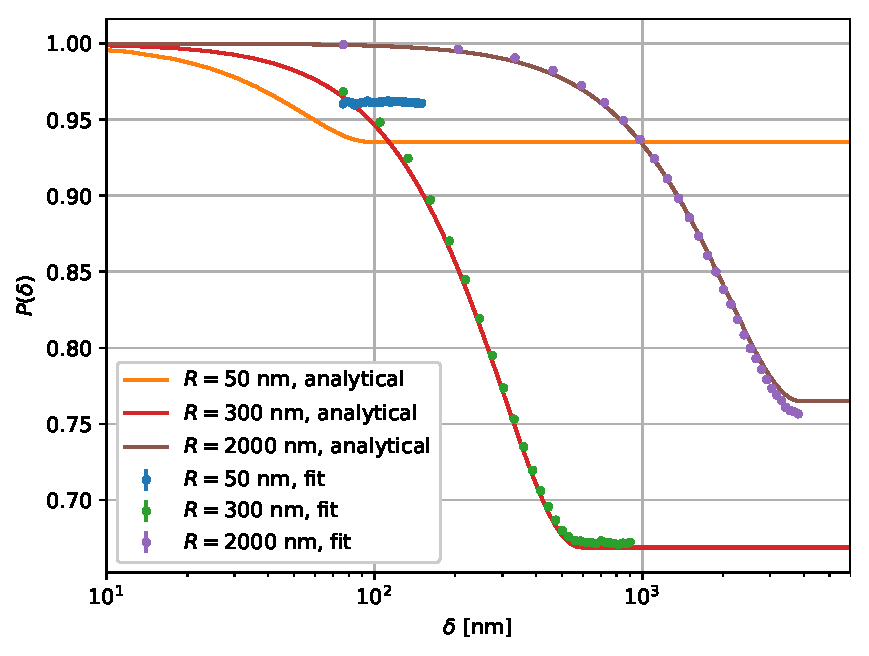
\includegraphics[width=\textwidth]{simulation-plot-gauss-FOIL-4.321}
		\caption{FOIL 4.321}
		\label{fig:simulation-plot-gauss-FOIL-4.321}
	\end{subfigure}
	\hfill
	\begin{subfigure}[b]{0.45\textwidth}
		\centering
		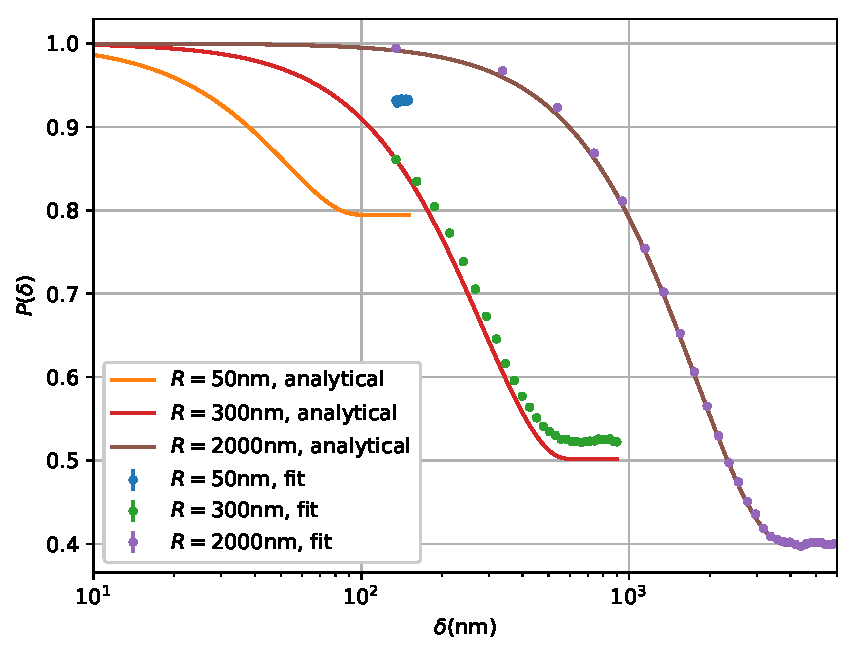
\includegraphics[width=\textwidth]{simulation-plot-gauss-FOIL-8}
		\caption{FOIL 8}
		\label{fig:simulation-plot-gauss-FOIL-8}
	\end{subfigure}
	\centering
	\begin{subfigure}[b]{0.45\textwidth}
		\centering
		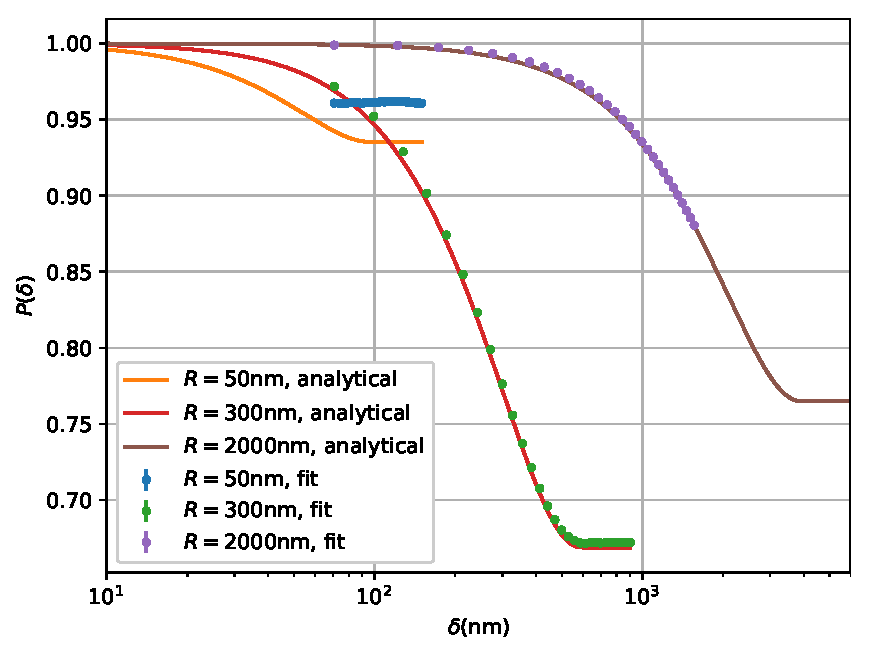
\includegraphics[width=\textwidth]{simulation-plot-gauss-WSP-4.321}
		\caption{WP 4.321}
		\label{fig:simulation-plot-gauss-WSP-4.321}
	\end{subfigure}
	\hfill
	\begin{subfigure}[b]{0.45\textwidth}
		\centering
		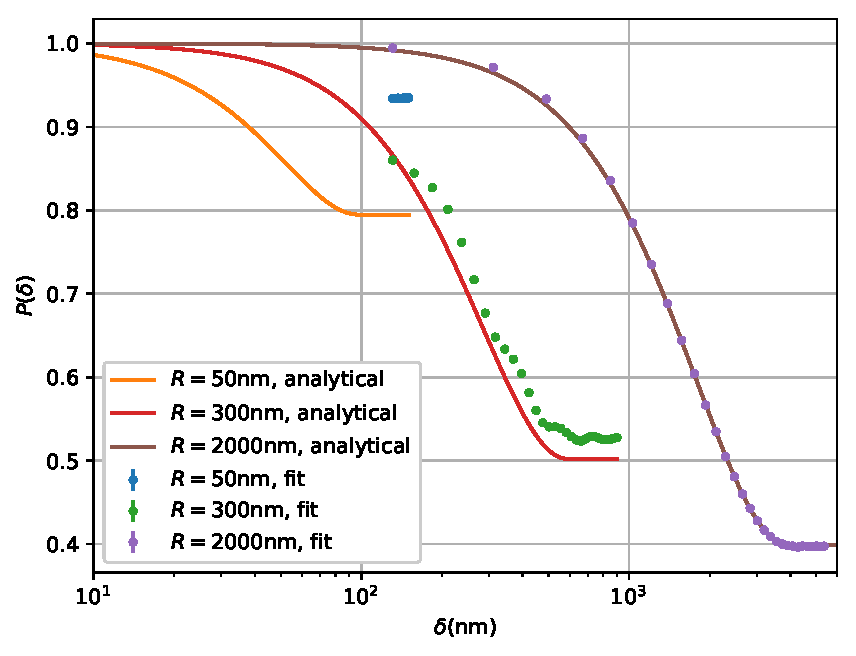
\includegraphics[width=\textwidth]{simulation-plot-gauss-WSP-8}
		\caption{WP 8}
		\label{fig:simulation-plot-gauss-WSP-8}
	\end{subfigure}
	\centering
	\begin{subfigure}[b]{0.45\textwidth}
		\centering
		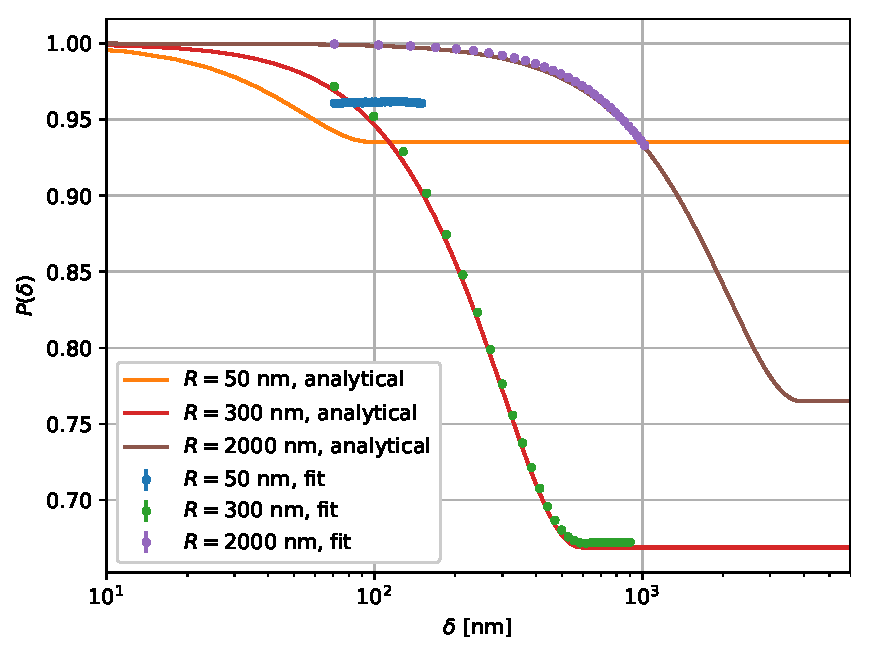
\includegraphics[width=\textwidth]{simulation-plot-gauss-ISO-4.321}
		\caption{ISO 4.321}
		\label{fig:simulation-plot-gauss-ISO-4.321}
	\end{subfigure}
	\hfill
	\begin{subfigure}[b]{0.45\textwidth}
		\centering
		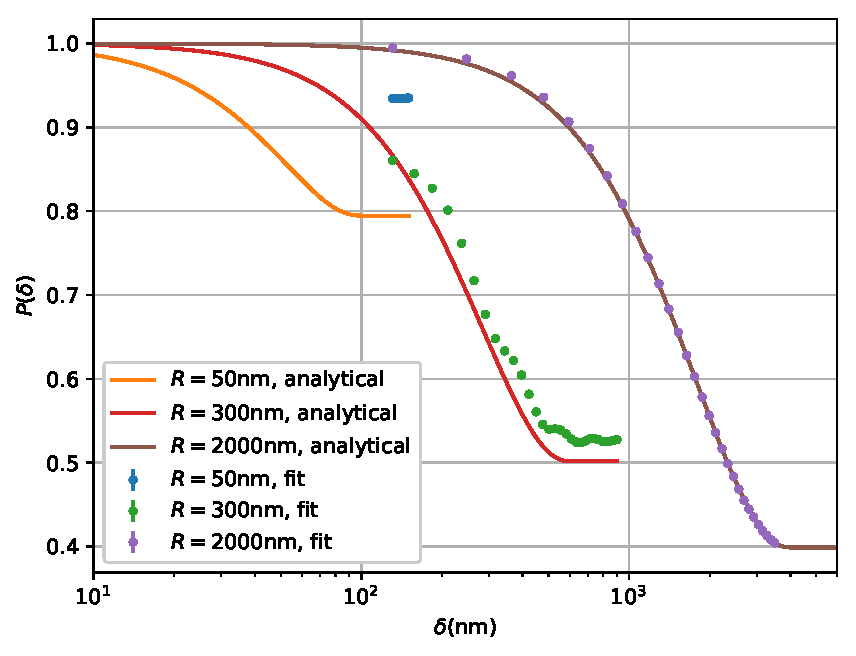
\includegraphics[width=\textwidth]{simulation-plot-gauss-ISO-8}
		\caption{ISO 8}
		\label{fig:simulation-plot-gauss-ISO-8}
	\end{subfigure}
	\caption{$P_{exp}(\delta)$ values derived from a fit of a Gaussian modulation envelope to detector intensity simulation data. Measurements using each of the six instruments were simulated using three samples as specified in Table \ref{tab:sample-thickness} together with the corresponding analytical $P(\delta)$. In most cases the error-bars are too small to be seen with exception of FOIL 4.321, FOIL 8, which were simulated using $10^7$ neutrons per measurement instead of $10^8$.}
	\label{fig:simulation-plot-gauss}
\end{figure}

\begin{figure}[p]
	\centering
	\begin{subfigure}[b]{0.45\textwidth}
		\centering
		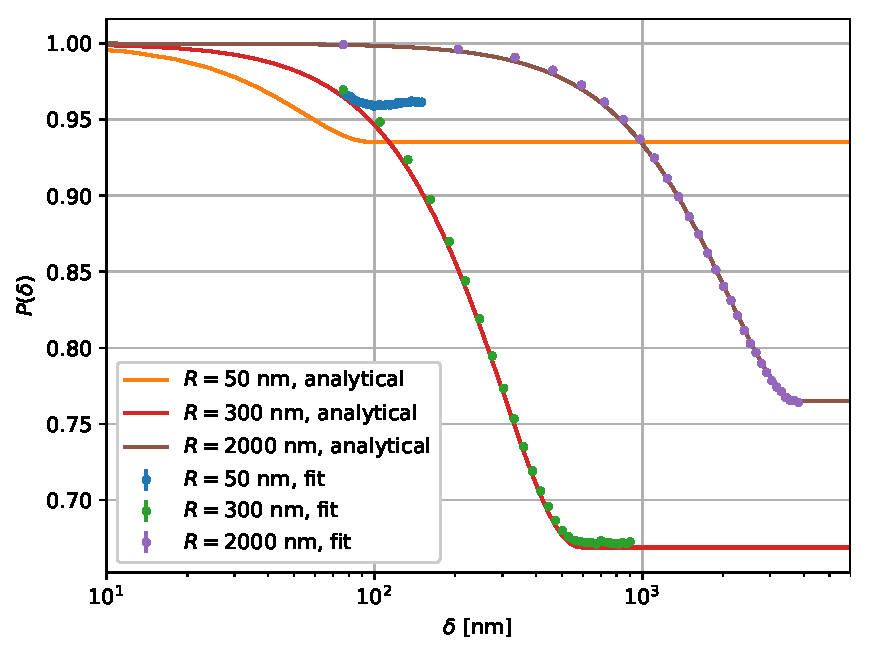
\includegraphics[width=\textwidth]{simulation-plot-rms-FOIL-4.321}
		\caption{FOIL 4.321}
		\label{fig:simulation-plot-rms-FOIL-4.321}
	\end{subfigure}
	\hfill
	\begin{subfigure}[b]{0.45\textwidth}
		\centering
		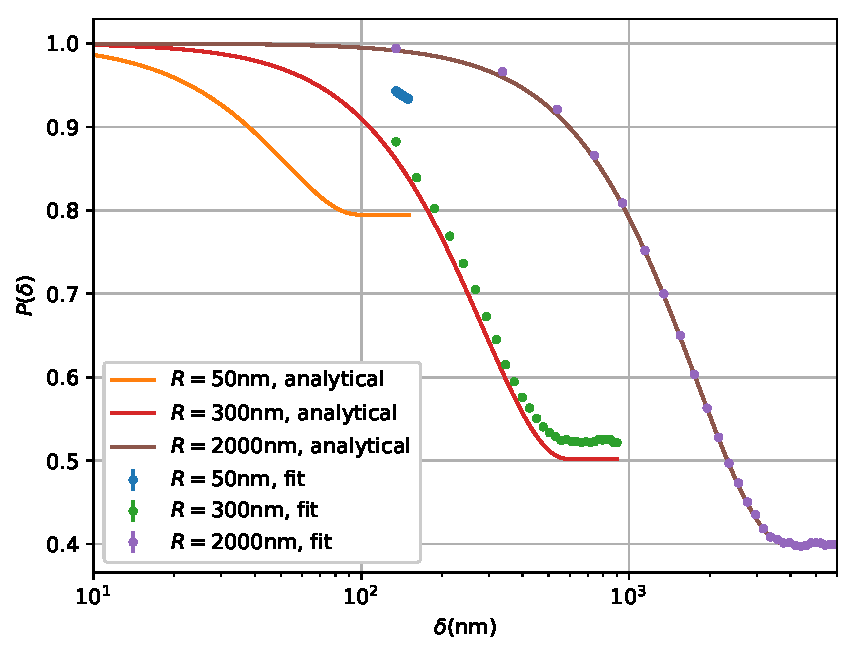
\includegraphics[width=\textwidth]{simulation-plot-rms-FOIL-8}
		\caption{FOIL 8}
		\label{fig:simulation-plot-rms-FOIL-8}
	\end{subfigure}
	\centering
	\begin{subfigure}[b]{0.45\textwidth}
		\centering
		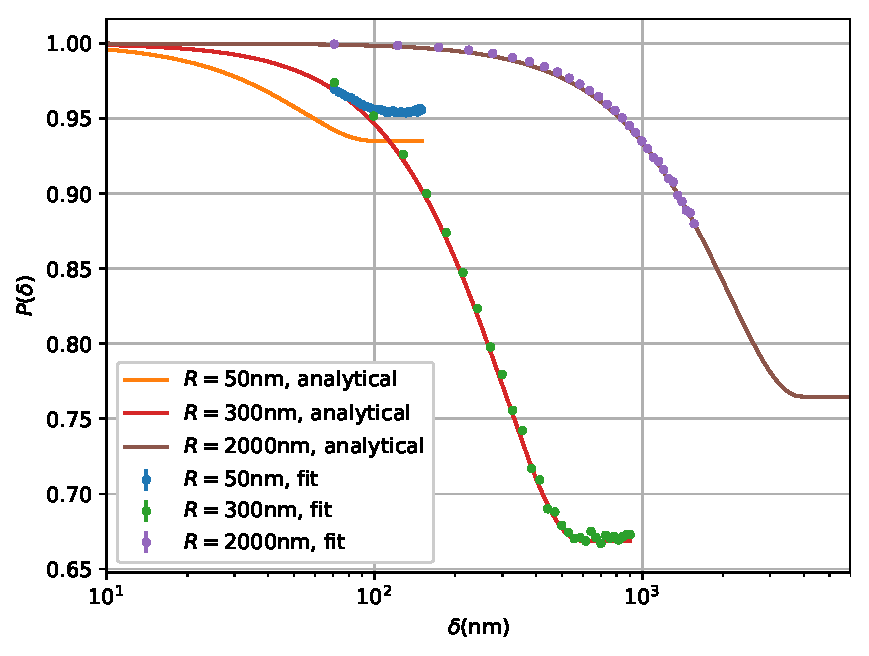
\includegraphics[width=\textwidth]{simulation-plot-rms-WSP-4.321}
		\caption{WP 4.321}
		\label{fig:simulation-plot-rms-WSP-4.321}
	\end{subfigure}
	\hfill
	\begin{subfigure}[b]{0.45\textwidth}
		\centering
		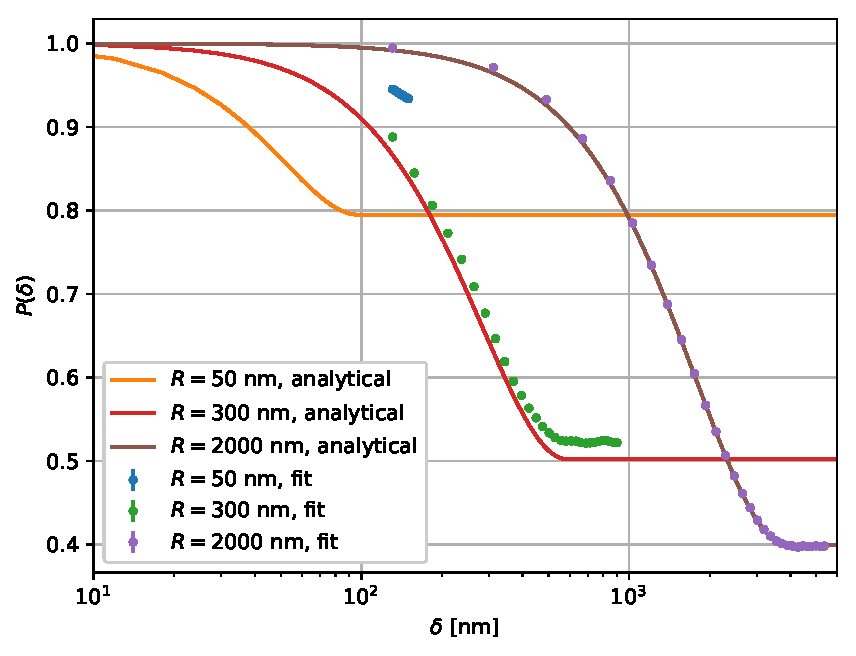
\includegraphics[width=\textwidth]{simulation-plot-rms-WSP-8}
		\caption{WP 8}
		\label{fig:simulation-plot-rms-WSP-8}
	\end{subfigure}
	\centering
	\begin{subfigure}[b]{0.45\textwidth}
		\centering
		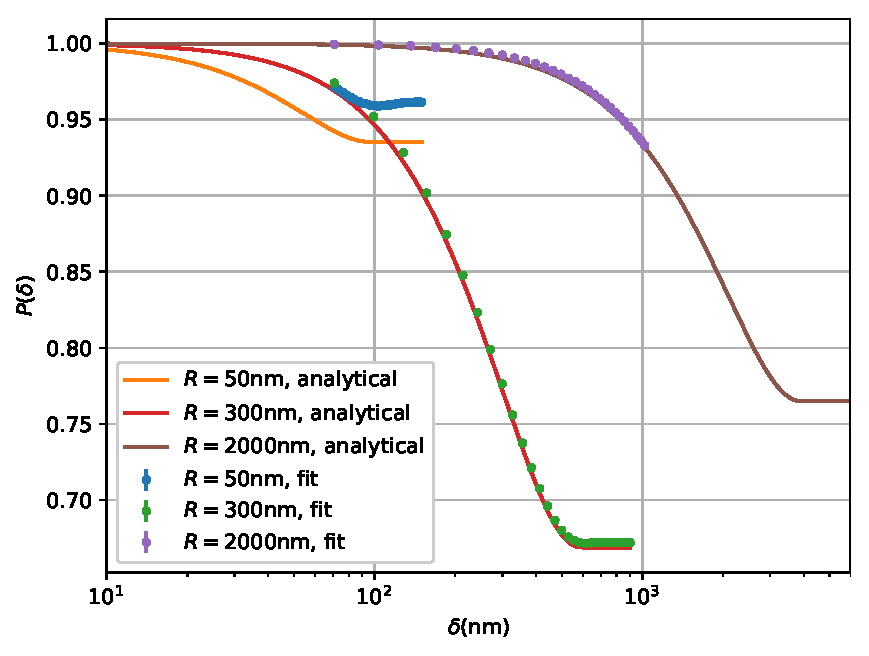
\includegraphics[width=\textwidth]{simulation-plot-rms-ISO-4.321}
		\caption{ISO 4.321}
		\label{fig:simulation-plot-rms-ISO-4.321}
	\end{subfigure}
	\hfill
	\begin{subfigure}[b]{0.45\textwidth}
		\centering
		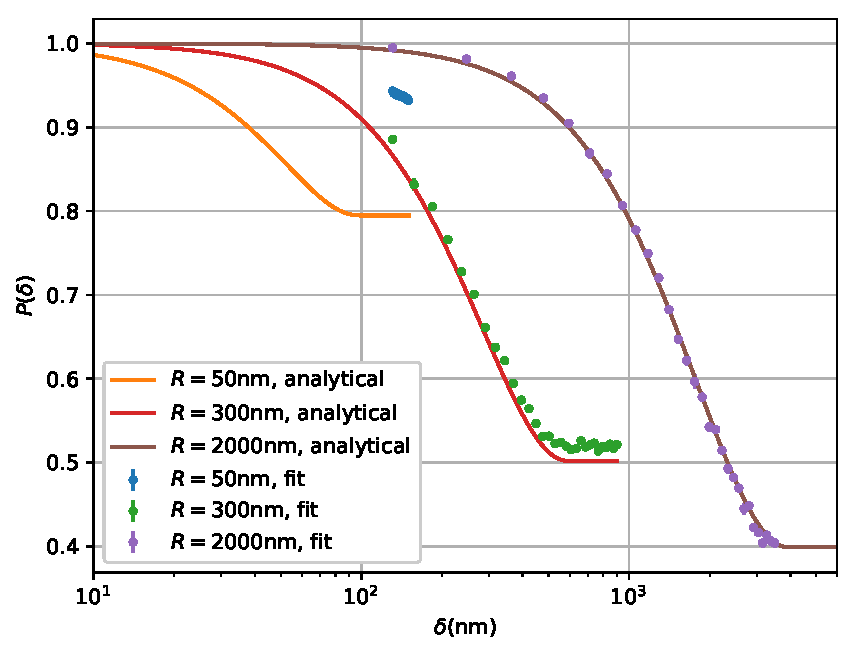
\includegraphics[width=\textwidth]{simulation-plot-rms-ISO-8}
		\caption{ISO 8}
		\label{fig:simulation-plot-rms-ISO-8}
	\end{subfigure}
	\caption{$P_{exp}(\delta)$ values derived using the RMS method together with analytical $P(\delta)$ curves for three different samples. The data is the same as shown in Figure \ref{fig:simulation-plot-gauss}.}
	\label{fig:simulation-plot-rms}
\end{figure}

\section{Discussion}
When comparing Figures \ref{fig:simulation-plot-gauss}, \ref{fig:simulation-plot-rms}, it appears that generally speaking both analysis methods give similar results. While the RMS method is more noise sensitive as can be seen from fits like Figure \ref{fig:simulation-plot-rms-FOIL-4.321} as compared to \ref{fig:simulation-plot-gauss-FOIL-4.321}, it seems to give more consistent results, giving a more reasonable fit of the $R=\SI{50}{\nano\meter}$ sample by appearing to capture some of the curvature of $P(\delta)$ in Figure \ref{fig:simulation-plot-rms-WSP-4.321}. Although corrections compensating for a too low detector $Q$-range \cite{kusmin2017} were not performed, it could be that the corrected analytical $P(\delta)$ curve for this sample looks somewhat like the $P_{exp}(\delta)$ fitted to data. Both methods also give a $P_{exp}(\delta)$ for $R = \SI{300}{\nano\meter}$ that is shifted upwards compared to the expected $P(\delta)$ for all instruments with $\lambda_0 = \SI{8}{\angstrom}$, indicating that $P_{exp}(\delta)$ probably accurately describes the fitted $y$-range of $Pol(y)$ data but cannot simply be said to estimate $P(\delta)$. Fitting only the middle $\SI{2}{\milli\meter}$ instead of the middle $\SI{6}{\milli\meter}$ of the detector reduces this error somewhat but not entirely. This can perhaps be explained by the relatively high $\tau = 0.6893$ as listed in Table \ref{tab:sample-thickness}, causing a relatively higher degree of multiple scattering and a larger fraction of scattered neutrons to go undetected making $P_{exp}(\delta)$ a poor estimate of $P(\delta)$. Another reason could be the greater $\Delta\lambda$ of designs at $\lambda_0 = \SI{8}{\angstrom}$, causing errors of the type discussed in Section \ref{c3.6} in addition to a greater spread scattering angles as $Q\propto 1/\lambda$, making the same $Q$ scatter into larger angles for higher $\lambda$, reducing the quality of estimate $P_{exp}(\delta)$ and the effective $Q$-range of the instrument.

This could mean that instruments with $\Delta\lambda/\lambda_0 = 0.1$ or similar like the three presented here with $\lambda_0 = \SI{8}{\angstrom}$ are more restricted for lower values of $\delta$ than predicted using the constraint model presented in Chapter \ref{c4:constraints} (which only considered $\Delta\lambda$ as having an effect on the modulation envelope), meaning that measuring wide $\delta$ ranges might be harder when using colder wavelengths available at a $T=\SI{20}{\kelvin}$ using a velocity selector. 

An alternative explanation would be that $P(\delta)$ needs to be corrected for the spread in $\lambda$ as discussed in Section \ref{c3.6}. This would also explain why the monochromatic $P(\delta)$ expression describes the fitted $P_{exp}(\delta)$ values well when $\Delta\lambda/\lambda_0 = 0.01$ but not when $\Delta\lambda/\lambda_0 = 0.1$. It is not clear what such a correction would look like. An alternative would be to use Fourier methods, but as indicated in Section \ref{c3.6} this can be complicated by frequency resolution constraints. 

% TODO add table illustrating different intensity

% None of the instruments were able to fully characterize the $R=50\unit{\nano\meter}$ sample, with the previously computed (hard) constraints listed limiting the $\delta$-range. 


%Although the instruments operating at $\lambda_0 = 4.321$Å were able to measure a somewhat wider range, all that can be said about these and those with $\lambda_0 = 8$Å is that they managed to estimate $P(\infty) = e^{-\tau}$ for this sample to differing degrees of accuracy. All instruments were able to measure the $R = 2000 \unit{\nano\meter}$ sample well within their given $\delta$ limitations, with all designs except WSP 4.321 and ISO 4.321 being able to measure up to $\delta \approx 2R$. Going by the analysis presented in Section \ref{c4.4}, it was expected that for $\lambda_0 = 4.321, 8$Å the approximate lower limit at which SEMSANS ceases to approximate $P(\delta)$ well is $100, 200\unit{\nano\meter}$ respectively. This appears to be reflected in the increasing error compared to the analytical expression for $R = 300\unit{\nano\meter}$ which has not been corrected for such an effect. The error is greater for $\lambda_0 = 8$Å which makes sense given what was discussed in Section \ref{c4.3}. This error can be reduced by fitting a smaller height than the centre $8\unit{\milli\meter}$, trading correctness of the estimate for increased uncertainty in $P(\delta)$, which can be understood by considering Figure \ref{fig:simplified-scattering} and the fraction of scattered neutrons that is 'missing' from each point on the detector. 

%\subsection{Comparison of analysis methods}
%When comparing Figures \ref{fig:simulation-plot-gauss}, \ref{fig:simulation-plot-rms}, it appears that generally speaking both analysis methods give similar results. While the RMS method is more noise sensitive as can be seen from fits like Figure \ref{fig:simulation-plot-rms-FOIL-4.321} as compared to \ref{fig:simulation-plot-gauss-FOIL-4.321}, it seems to give more consistent results, giving a more reasonable fit of the $R=50\unit{\nano\meter}$ sample by appearing to capture some of the curvature of $P(\delta)$. Although corrections compensating for a too low detector $Q$-range \cite{kusmin2017} were not performed, it could be that the corrected analytical $P(\delta)$ curve for this sample looks somewhat like what is fitted. 

% Did the simulations match the precomputed limits? Are the limits (to the extent that they are not absolute but rather somewhat chosen heuristically) good enough, too strict? Is it in practice possible to measure even at field strenghts outside of the range?